\documentclass[11pt,a4paper]{article}
\usepackage{amsmath}
\usepackage{amsfonts}
\usepackage{amssymb}
\usepackage{fancyhdr}
\usepackage{lastpage}
\usepackage{graphicx}
\usepackage{ucs}
\usepackage[utf8x]{inputenc}
\usepackage[italian]{babel}
\usepackage[colorlinks=true,linkcolor=black]{hyperref}

\renewcommand{\headrulewidth}{0.6pt}
\renewcommand{\footrulewidth}{0.6pt}
% impostazione dello stile per le pagine interne del documento
\lhead{\leftmark}
\chead{}
\rhead{
\includegraphics[scale=0.15]{logo.png} }
\lfoot{Specifica tecnica v0.3.1}
\cfoot{}
\rfoot{\thepage \ di \pageref{LastPage}}
% ridefinizione dello stile plain per il frontespizio
\fancypagestyle{plain}{
\fancyhf
}
% impostazione dello stile per l'indice
\fancypagestyle{indice}{
\lhead{\leftmark}
\chead{}
\rhead{
\includegraphics[scale=0.15]{logo.png}}
\lfoot{Specifica tecnica v0.3.1}
\cfoot{}
\rfoot{}
}
\headheight = 46pt
%definizione del comando "\modifiche" per la creazione del diario delle modifiche
\newcommand{\modifiche} 
{
\newpage
\begin{center}
\textbf{Diario delle modifiche} \\
\bigskip
\begin{tabular}{|c|c|p{0.62\textwidth}|}
\hline
\textsc{Data} & \textsc{Versione} & \textsc{Modifica} \\
\hline
\hline
\textit{23-01-2009} & 0.3.1 & Correzioni varie \\
\hline
\textit{22-01-2009} & 0.3.0 & Aggiunti i flussi di esecuzione \\
\hline
\textit{21-01-2009} & 0.2.0 & Stesura Descrizione dei componenti \\
\hline
\textit{20-01-2009} & 0.1.0 & Creazione dell'indice \\
\hline
\end{tabular}
\end{center}
}
%definizione del comando "\info" per la creazione delle informazioni del documento
\newcommand{\info} {
\bigskip
\begin{tabbing}
	\hspace*{0.3\textwidth} \= \hspace*{0.5\textwidth} \kill
	\parbox{0.3\textwidth}{\textbf{Verifica: }} \> \parbox{0.5\textwidth}{Freo Matteo} \\
	\parbox{0.3\textwidth}{\textbf{Approvazione: }} \> \parbox{0.5\textwidth}{Scortegagna Carlo} \\
	\parbox{0.3\textwidth}{\textbf{Stato: }} \> \parbox{0.5\textwidth}{Formale} \\
	\parbox{0.3\textwidth}{\textbf{Uso: }} \> \parbox{0.5\textwidth}{Esterno} \\
	\parbox{0.3\textwidth}{\textbf{Distribuzione: }} \> \parbox{0.5\textwidth}{QuiXoft} \\
							\> \parbox{0.5\textwidth}{Rossi Francesca} \\
							\> \parbox{0.5\textwidth}{Vardanega Tullio} \\
							\> \parbox{0.5\textwidth}{Conte Renato} \\
\end{tabbing}
}
%definizione del comando "\frontespizio" per la creazione del frontespizio
\newcommand{\frontespizio} {
\thispagestyle{plain}
\title{\begin{Huge}\textsc{Progetto SIGEOL}\end{Huge} \\ \textit{Specifica Tecnica \\ v0.3.1}}
\author{Redazione: }
\maketitle
\medskip
\begin{center}

\includegraphics[scale=0.5]{logo.png} \\
\textit{quixoft.sol@gmail.com}
\end{center}
\medskip
\info
\begin{center}
\textbf{Sommario} \\
Documento contenente la specifica tecnica per il progetto ''SIGEOL'' commissionato dalla prof. Rossi Francesca.
\end{center}
\newpage
}
%definizione del comando "\indice" per la creazione dell'indice
\newcommand{\indice} {
\thispagestyle{indice}
\tableofcontents
\newpage
}
\pagestyle{fancy}
\begin{document}
\frontespizio
\indice
\setcounter{page}{1}
\section{Introduzione}
\subsection{Scopo del documento}
Il presente documento denominato \textsc{Specifica tecnica} ha lo scopo di mostrare la struttura del progetto \textit{SIGEOL} e descrivere i componenti che ne fanno parte. 
\subsection{Scopo del prodotto}
Il progetto sotto analisi, denominato \textit{SIGEOL}, si prefigge di automatizzare la generazione, la gestione, l'ottimizzazione e la consultazione degli orari di lezione. 
\subsection{Glossario}
Le definizioni dei termini specialistici usati nella stesura di questo e di tutti gli altri documenti possono essere trovate nel documento \textsc{Glossario} al fine di eliminare ogni ambiguità e di facilitare la comprensione dei temi trattati. Ogni termine la cui definizione è disponibile all’interno del Glossario verrà marcato con una \underline{sottolineatura}.

\section{Definizione del prodotto}
\subsection{Metodo e formalismo di specifica}
Lo strumento principale nel redarre la specifica tecnica sarà il linguaggio \underline{UML}, che permetterà di realizzare i diagrammi delle classi, di sequenza, di collaborazione e di attività.


La decomposizione architetturale utilizzata sarà di tipo \underline{Top-down}.
E' prevista una descrizione generale dell’architettura del sistema, alla quale seguiranno le specifiche dettagliate dei suoi componenti.


Per semplificare la progettazione, si utilizzeranno i seguenti pattern:
\begin{description}
 \item[\textbf{MVC}] 
Il pattern MVC (Model View Controller) si basa sulla separazione tra i componenti software del sistema, che gestiscono il modo in cui presentare i dati, e i componenti che gestiscono i dati stessi. 
 \item[\textbf{Façade}]
Permette, attraverso un'interfaccia più semplice, l'accesso a sottosistemi aventi interfacce complesse e molto diverse tra loro, nonché a blocchi di codice complessi.
\item[\textbf{REST}]
Representational state transfer (REST) è un tipo di architettura software per i sistemi di ipertesto distribuiti come il World Wide Web. 
REST si riferisce ad un insieme di principi di architetture di rete, i quali delineano come le risorse sono definite e indirizzate.


\item[\textbf{Convention Over Configuration}]
Convention Over Configuration è un paradigma di programmazione che prevede configurazione minima (o addirittura assente) per il programmatore che utilizza un framework che lo rispetti, obbligandolo a configurare solo gli aspetti che si differenziano dalle implementazioni standard o che non rispettano particolari convenzioni di denominazione o simili.
Significa che Rails prevede delle impostazioni di default per qualsiasi aspetto dell’applicazione. Utilizzando queste convenzioni sarà possibile velocizzare i tempi di sviluppo evitando di realizzare scomodi file di configurazione. L’esempio più chiaro del COC si può notare a livello di modelli: rispettando le convenzioni previste dal framework è possibile realizzare strutture di dati complesse con molte relazioni tra oggetti in pochissimo tempo, in maniera quasi meccanica e soprattutto senza definire nessuna configurazione. Questo concetto differenzia Rails dai framework che prevedono molte righe di configurazione per ogni aspetto dell’applicazione. Con il COC tutto diventa più snello e più dinamico. Ovviamente per situazioni in cui le convenzioni non possano essere rispettate, Rails permette di utilizzare schemi funzionali diversi da quelli previsti.
\item[\textbf{DRY}]
Questo concetto, fortemente filosofico, prevede che ciascun elemento di un’applicazione debba essere implementato solamente una volta e niente debba essere ripetuto. Questo significa che, mediante Rails, è possibile gestire funzionalità ripetitive con una estrema fattorizzazione del codice (''scrivo una volta e uso più volte'') che facilita sia lo sviluppo iniziale che eventuali modifiche successive del prodotto.
\item[\textbf{View Helper}]
Questo pattern disaccoppia il Business Logic dallo strato View, il che facilita
la manutenibilità. Aiuta a separare, in fase di sviluppo, la responsabilità
del web designer e dello sviluppatore.
\item[\textbf{Active Record}]
Secondo il pattern Active Record esiste una relazione molto stretta fra tabella e classe, colonne e attributi della classe. 
\begin{itemize}
 \item una tabella di un database relazionale è gestita attraverso una classe
\item una singola istanza della classe corrisponde ad una riga della tabella
\item alla creazione di una nuova istanza viene creata una nuova riga all'interno della tabella, e modificando l'istanza la riga viene aggiornata
\end{itemize}
\end{description}


Il sistema verrà implementato utilizzando Ruby on rails, un framework la cui architettura è fortemente ispirata al paradigma Model-View-Controller. 
Oltre a veicolare lo sviluppo di applicazioni secondo il pattern MVC, il RESTful Rails impone un’ulteriore disciplina nella codifica che garantisce maggiore compattezza, migliore leggibilità, “pretty-urling” e semplicità nella costruzione di API.

\subsection{Presentazione dell'architettura generale del sistema}
Per presentare l'architettura generale del sistema \textit{Sigeol} si utilizzerà il pattern Model-View-Controller(MVC).
In questo modello i ruoli di presentazione, controllo ed accesso ai dati vengono affidati a componenti diversi e sono tra di loro disaccoppiati.


\begin{center}
 \textbf{View}
\end{center}
E' il primo livello che si incontra e contiene i componenti che costituiscono l'interfaccia grafica, tramite la quale l'utente interagisce con il sistema \textit{Sigeol}.
La View delega al Controller l'esecuzione dei processi richiesti dall'utente dopo averne catturato gli input e la
scelta delle eventuali schermate da presentare.
ActionView gestisce l'aspetto delle pagine da restituire al client. Sono per lo più file .rhtml che contengono delle direttive scritte in Ruby immerse nel codice XHTML.

\begin{center}
 \textbf{Model}
\end{center}
Definisce i dati e le operazioni che possono essere eseguite su questi. Quindi definisce le regole di business per l'interazione con i dati, esponendo alla View ed al Controller rispettivamente le funzionalità per l'accesso e l'aggiornamento.
Viene gestito da una libreria chiamata ActiveRecord, che si occupa di tutta la logica di business e che permette l'accesso a numerosi DataBase bastati su SQL. Con questa libreria si stabilisce un collegamento tra le classi scritte in Ruby e le tabelle del DB.

\begin{center}
 \textbf{Controller}
\end{center}
Questo componente ha la responsabilità di trasformare le interazioni dell'utente della View in azioni eseguite dal Model. Ma il Controller non rappresenta un semplice "ponte" tra View e Model. Realizzando la mappatura tra input dell'utente e processi eseguiti dal Model e selezionando le schermate della View richieste, il Controller implementa la logica di controllo dell'applicazione.

Gestisce le richieste del browser e facilita la comunicazione fra Model e View. Tutti i controller creati dall'utente ereditano da ActionController. L'ApplicationController raccoglie funzionalità condivise nell'intera applicazione.
In particolare verranno inserite le azioni CRUD (Create-Read-Update-Delete) per l'oggetto e le varie funzioni che possono servirci per la nostra applicazione.
I Controller sono gestiti dal componente ActionController che fa parte del pacchetto di moduli rails chiamato Action Pack.
I Controller sono rappresentati dalla libreria ActionController.
Gestisce le richieste del browser e facilita la comunicazione fra Model e View. Tutti i controller creati dall'utente ereditano da ActionController. L'ApplicationController raccoglie funzionalità condivise nell'intera applicazione.
In particolare verranno inserite le azioni CRUD (Create-Read-Update-Delete) per l'oggetto e le varie funzioni che possono servirci per la nostra applicazione.
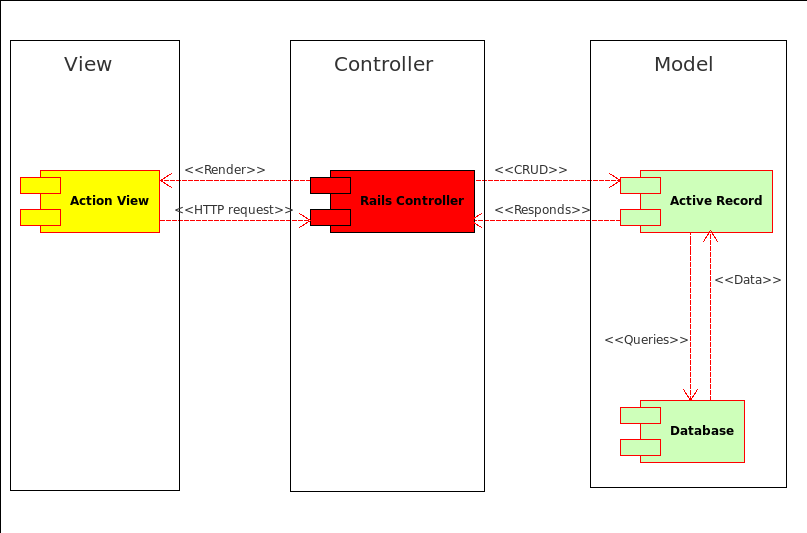
\includegraphics[scale=0.50]{images/SIGEOL.png}


\section{Descrizione dei singoli componenti}
\subsubsection{Parte Controller}
\begin{center}
 \textbf{Action Controller}
\end{center}
Il modulo che gestisce la parte controller è contenuto all'interno del framework Ruby on rails ed è chiamato Action Controller.
Questo, assieme all'Action View(vedi Parte view) è integrato all'interno di un pacchetto chiamato Action Pack.
%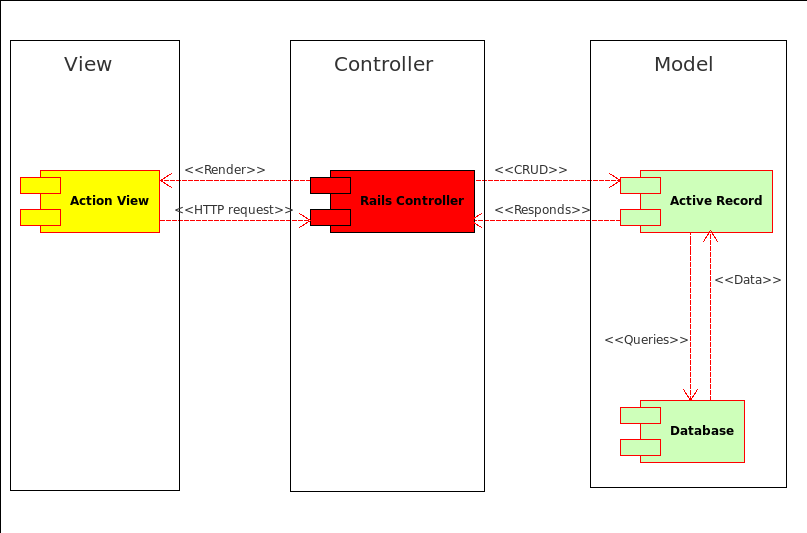
\includegraphics[scale=0.50]{images/SIGEOL.png}


Ogni controller è una normale classe, ed ogni metodo pubblico definito in questa classe corrisponde ad un'azione specifica.
Ad ogni azione definita corrisponde una vista. 

Ruby on Rails riconosce il tipo di richiesta pervenuta codificando le informazioni all'interno di un URL e si serve di un componente chiamato Rounting, per determinare l'azione cui deve essere sottoposta la richiesta.
Il componente \textbf{Routing} traccia una mappatura che permette a Rails di collegare gli URL esterni e l'azione contenuta in una determinata classe Controller.


Ad esempio, Dato un URL nel formato \textit{nomecontroller/azione/id}, viene identificato il Controller \textit{nomecontroller} e viene istanziato. A questo punto l'oggetto richiama il metodo con nome \textit{azione} e con parametro \textit{id}. Il Controller infine cercherà di visualizzare un template con lo stesso nome dell'azione. 

\subsubsection{Parte View}
\begin{center}
 \textbf{Action View}
\end{center}
 Il modulo Action View contenuto nel framework Ruby on Rails, offre meccanismi avanzati per il riutilizzo del codice, tramite l'uso di viste e di metodi helper pensati per generare ad esempio pagine XHTML.
I metodi helper sono semplici metodi pubblici di una classe Controller.

\subsubsection{Parte Model}
L'ActiveRecord è il modulo di Ruby on Rails che gestisce la persistenza dei dati. 
Il modulo è stato implementato seguendo il pattern Active Record facendo largo uso di convenzioni sui nomi da assegnare a tabelle, classi, colonne e attributi; se non sono presenti configurazioni particolari del modello, sono valide le seguenti convenzioni:
\begin{itemize}
 \item per ogni modello esiste una tabella avente come nome il nome del modello al plurale e in caratteri minuscoli;
\item nel caso di modelli con nome composto di più parole, il nome del modello ha la prima lettera di ogni parola; maiuscola, mentre la tabella ha sempre il nome tutto in minuscolo e separa le parole con un trattino basso (underscore);
\item per ogni colonna della tabella viene reso disponibile il relativo attributo con lo stesso nome;
\item ogni tabella ha una colonna id (intero positivo) che identifica univocamente ogni record;
\end{itemize}
La classe è descritta in buona parte dalla tabella che rappresenta ed espone i metodi necessari per leggere e scrivere i record.
Con ActiveRecord è possibile utilizzare diversi tipi di database: SQLite, MySQL, Postgresql, Oracle, IBM DB/2 ed è possibile scrivere driver personalizzati per altri database relazionali.

\subsection{Relazioni d'uso di altre componenti}
\subsection{Interfacce con e relazioni di uso da altre componenti}
\subsection{Attività svolte e dati trattati}
\section{Stime di fattibilità e di bisogno di risorse}
\section{Tracciamento della relazione componenti-requisiti}
\section{Flusso di esecuzione}
La seguente sezione si fa carico di illustrare, con l'utilizzo di diagrammi di attività, i flussi delle varie azioni che gli utenti del sistema SIGEOL hanno la possibilità di compiere.
Quanto riportato in seguito è da considerarsi passibile di modifiche col procedere della fase di progettazione.
\newpage
\subsection{Login utenti}
La Segreteria Didattica e tutti Docenti registrati hanno la possibilità di accedere alla pagina di login per inserire le proprie credenziali ed accedere alle funzioni aggiuntive che il sistema SIGEOL mette loro a disposizione. Il Presidente del CCS viene considerato un Docente, ma con in più la possibilità di accedere a tutte le funzioni tipiche della Segreteria Didattica.

Al termine della fase di login, l'utente verrà reindirizzato alla pagina principale di SIGEOL e potrà espletare le funzioni a sua disposizione.\\
\begin{center}
 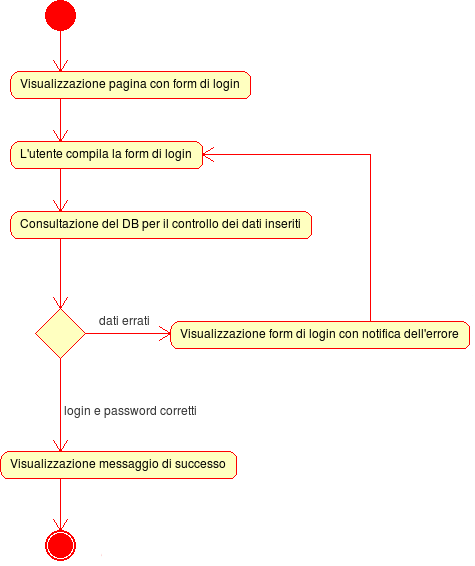
\includegraphics[scale=1]{images/login.png}
\end{center}

\newpage
\subsection{Inserimento nuovo Docente}
La Segreteria Didattica e il Presidente del CSS hanno la possibilità, dopo aver effettuato con successo il login, di inserire un nuovo Docente nel sistema SIGEOL. Verranno richiesti nome, cognome ed indirizzo email. Se tali dati vengono inseriti e il Docente non è già presente nel DB di sistema, viene automaticamente inviata una email al Docente invitato, in cui gli viene indicato il link necessario per procedere alla creazione del suo account.
\begin{center}
 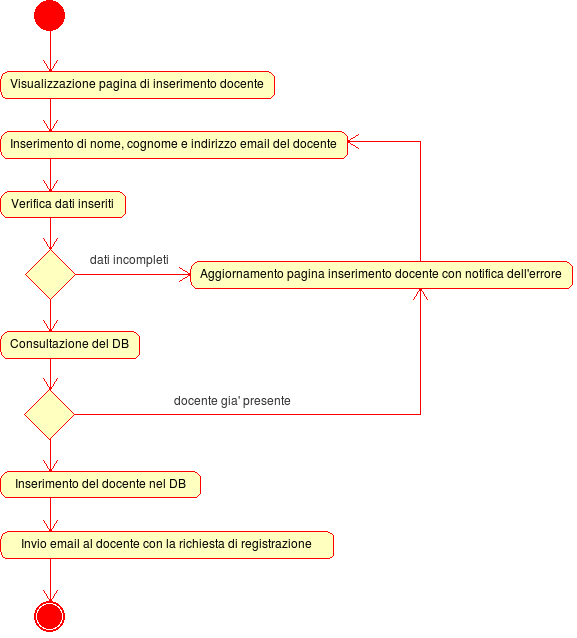
\includegraphics[scale=0.9]{images/inserimento_docente.png}
\end{center}

\newpage
\subsection{Registrazione Docente}
Ogni docente, dopo aver ricevuto la mail di invito al sistema SIGEOL, utilizza il link ricevuto per accedere al form di scelta password e di inserimento degli altri dati personali. La scelta della password seguirà rigide regole di sintassi, che verranno controllate dinamicamente durante l'inserimento. Tali regole prevederanno un numero minimo di caratteri, la presenza obbligatoria di cifre o simboli e altre convenzioni che saranno decise dal team QuiXoft, in collaborazione con il Committente, durante il proseguimento della fase di progettazione. La password dovrà poi essere confermata in un successivo campo dati, per evitare spiacevoli errori di battitura.

Al termine della prcedura la password scelta e gli altri dati inseriti verranno memorizzati in modo sicuro sul DB di sistema.
\begin{center}
 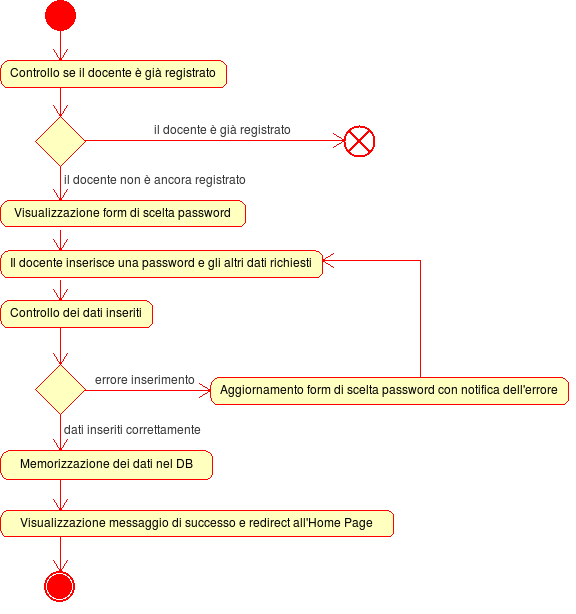
\includegraphics[scale=0.8]{images/registrazione_docente.png}
\end{center}

\newpage
\subsection{Inserimento dei dati nel sistema}
La Segreteria Didattica e il Presidente del CCS hanno la possibilità di inserire i dati relativi ai corsi di laurea, agli insegnamenti, alle aule, ai dipartimenti e molti altri dati indispensabili al funzionamento del sistema SIGEOL.

L'inserimento avverrà tramite diverse pagine web e diverse form, ma il diagramma di flusso di tali inserimenti è cosi simile che è stato scelto di esporne solo uno generale, adatto a rappresentare tutti gli inserimenti.
\begin{center}
 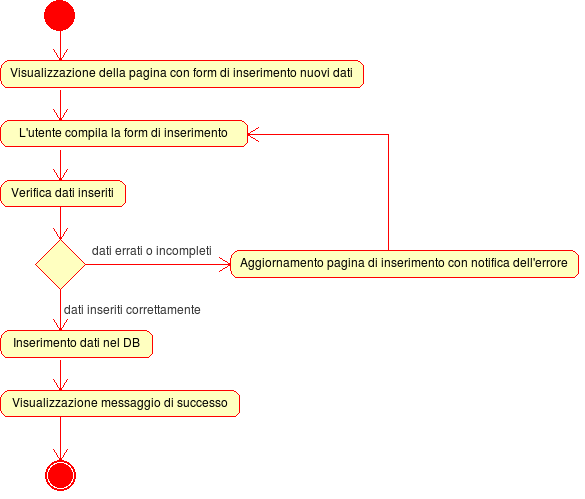
\includegraphics[scale=0.85]{images/inserimento_dati.png}
\end{center}

\newpage
\subsection{Modifica dei dati del sistema}
La Segreteria Didattica e il Presidente del CCS hanno la possibilità di modificare tutti i dati relativi ai corsi di laurea, agli insegnamenti, alle aule, ai dipartimenti, ecc...

I docenti invece hanno la possibilità di modificare i propri dati personali e i vincoli e le preferenze inserite.

Le similitudini tra tutte le sopra citate modifiche hanno portato allo sviluppo di un singolo diagramma di attività che le rappresenti tutte. L'invocazione del comando di modifica sarà ovviamente diverso tra i vari tipi di dati, ma la procedura per modificarli e salvarli è similare.

\begin{center}
 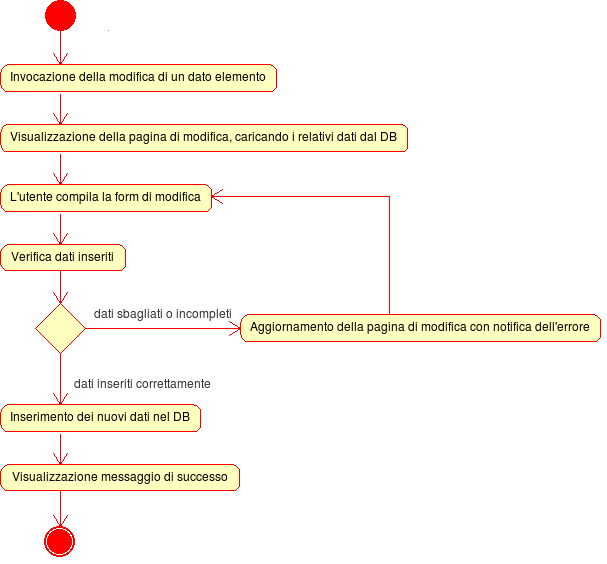
\includegraphics[scale=0.85]{images/modifica_dati.png}
\end{center}

\newpage
\subsection{Inserimento vincoli e preferenze da parte dei Docenti}
Tutti i docenti cha abbiano effettuato correttamente il login hanno la possibilità di inserire i loro vincoli e le loro preferenze. La procedura è similare, per tanto è rappresentata dallo stesso diagramma di attività.

La differenza sostanziale nell'inserimento di un vincolo o di una preferenza è che solo il vincolo, tra i due, prevede una motivazione, mentre solo la preferenza prevede un livello di priorità. L'assegnazione della priorità di una preferenza è automatizzata dal sistema: il Docente dovrà solamente decidere l'ordine di importanza delle proprie preferenze.

\begin{center}
 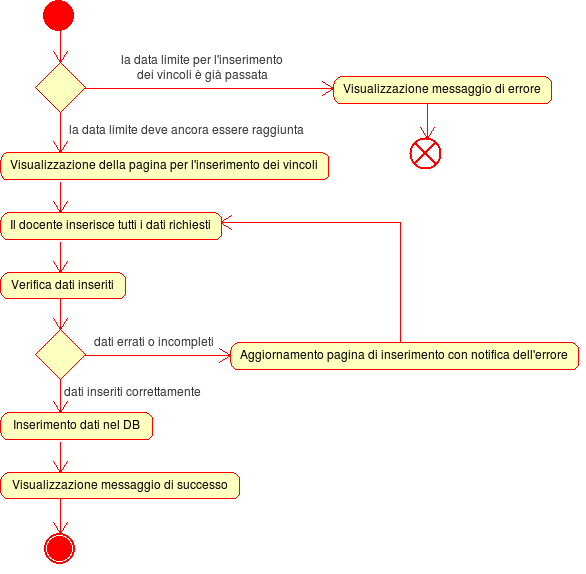
\includegraphics[scale=0.85]{images/inserimento_vincoli.png}
\end{center}

\newpage
\subsection{Generazione dell'orario}
La Segreteria Didattica e il Presidente del CCS hanno la possibilità, una volta scaduta la data limite per l'inserimento dei vincoli e delle preferenze da parte dei Docenti, di far partire l'algoritmo di generazione dell'orario. L'algoritmo calcolerà l'orario migliore possibile per tutti i Corsi di Laurea inseriti, e sarà data la possibilità di scelta se generare l'orario per uno o più periodi (per periodo si intende il numero di trimestre-semestre-ecc... in base alla scelta fatta nel momento di inserimento dei dati).

L'algoritmo proporrà un orario soddisfacendo tutti i requisiti presenti e tentando di rispettare il più possibile tutte le preferenze. Se ciò non fosse possibile, sarà data la possibilità alla Segreteria Didattica o al Presidente del CCS di rilassare certi vincoli o di modificare manualmente lo schema d'orario generato.
\begin{center}
 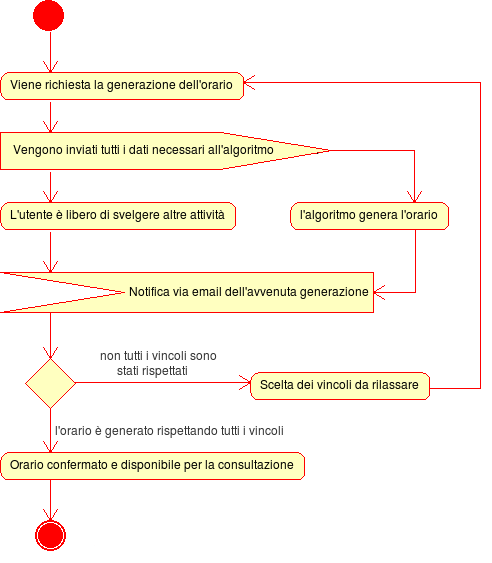
\includegraphics[scale=0.85]{images/generazione_orario.png}
\end{center}


\modifiche
\end{document}
